\documentclass[12pt,a4paper]{article}

% load packages
\usepackage{xcolor}
\usepackage{graphicx}
\usepackage{amsmath}
\usepackage{amsfonts}
\usepackage{amssymb}
\usepackage{listings}
\usepackage{hyperref}
\usepackage{algorithm}
\usepackage{algpseudocode}
\usepackage{float}
\usepackage{tabularx}
\usepackage{multirow}
\usepackage{booktabs}
\usepackage{setspace}
\setstretch{1.1}
\usepackage{appendix}
\usepackage[left=2cm,right=2cm,top=2cm,bottom=2cm]{geometry}

% set code style
\definecolor{codegreen}{rgb}{0,0.6,0}
\definecolor{codegray}{rgb}{0.5,0.5,0.5}
\definecolor{codepurple}{rgb}{0.58,0,0.82}
\definecolor{backcolour}{rgb}{0.95,0.95,0.92}


\title{Project 3 Report for Probelm 3.1}
\author{Zhu Liang}
\date{\today}

\begin{document}

\maketitle

\section{Project Description}
The primary objective of this project is to implement matrix multiplication using the Ring (a.k.a. Cannon)
 algorithm.
The performance of this method is then evaluated across varying matrix sizes and numbers of processors.
The program is implemented in C and compiled by the shell script \texttt{test.sh}.

The initial results from the main segment hints at potential cache effects influencing the performance metrics. 
To offer a clearer and unbiased perspective on the algorithm's performance, additional tests were conducted, 
aiming to minimize this cache influence. 
These supplementary tests and their outcomes are detailed in Appendix.



\section{Algorithm Description}
\begin{algorithm}[htbp]
    \caption{Ring Algorithm for Matrix Multiplication}
    \label{alg:ring}
    \begin{algorithmic}[1]
    \Procedure{RingMatrixMultiply}{$N, P, A, B$}
    \State \textbf{Initialize} MPI with rank and size $P$
    \State \textbf{Determine} local matrix sizes based on $N$ and $P$
    \State \textbf{Transpose} matrix $B$
    \State \textbf{Scatter} matrix $A$ and $B$ to all processor from \textit{root}
    \For{each rotation, all processors}
        \State \textbf{Perform} local matrix multiplication of $A$ and $B$
        \State \textbf{Store} current results on local $C$ matrix
        \State \textbf{Shift} local $B$ matrix to the left by one processor
    \EndFor
    \State \textbf{Gather} all local results to \textit{root}
    \If{rank is \textit{root}}
        \State \textbf{Formulate} the final result matrix and return
    \Else
        \State Return NULL
    \EndIf
    \EndProcedure
    \end{algorithmic}
\end{algorithm}


Matrix multiplication is a cornerstone in numerous computational tasks. 
Efficiently parallelizing this operation can considerably expedite computations,  
 particularly with large matrices. The ring algorithm offers a parallel approach for this. 
At its core, the algorithm scatters matrices across multiple processors. 
During each iteration, each processor computes a local multiplication, 
stores the result, and then shifts its portion of matrix to the neighboring processor. 
This rotation strategy ensures that each processor multiplies with all parts 
 of the other matrix over several iterations. 
The pesudocode for this algorithm is shown in Algorithm \ref{alg:ring}.



It's worth noting that this specific implementation slightly deviates from what's typically taught in class. 
Instead of rotating matrix $A$, we opt to rotate matrix $B$. 
This choice was driven by the convenience it provides in gathering the final result matrix 
 using the \texttt{MPI\_Gather} function under our costomized matrix data structure.

This description is intentionally streamlined, 
omitting many details and supporting functions for brevity. 
More details can be gleaned from the source code file \texttt{functions.c}.

\section{Results}
\subsection{Performance}

\begin{table}[ht]
    \centering
    \begin{tabular}{ccccccc}
        \toprule
        & \multicolumn{3}{c}{Ring Algorithm} & \multicolumn{1}{c}{} & \multicolumn{1}{c}{Naive Algorithm} \\
        \cmidrule(lr){2-4} \cmidrule(lr){6-6}
        (in seconds) & \( P = 2^2 \) & \( P = 2^4 \) & \( P = 2^6 \) & & \( P = 1 \) \\
        \midrule
        \( N = 2^8 \)  & 0.020182 & 0.006294 & 0.003478 & & 0.090545 \\
        \( N = 2^{10} \) & 1.163175 & 0.310421 & 0.095925 & & 6.119090 \\
        \( N = 2^{12} \) & 73.364430 & 18.900791 & 5.574106 & & 707.989130 \\
        \bottomrule
    \end{tabular}
    \caption{Performance of the Ring and Naive methods.}
    \label{tab:results}
\end{table}

As demonstrated in Table \ref{tab:results}, 
the performance of the Ring and Naive matrix multiplication methods is outlined for different matrix sizes (\(N\)) 
 and varying number of processors (\(P\)). 
The results indicate the time taken by each method to complete the matrix multiplication 
 for the specified configurations.

\subsection{Speedup}
Speedup is a metric that quantifies the performance improvement of a parallel algorithm compared to its sequential counterpart. 
The speedup \( S \) for \( P \) processors for size $N$ problem is defined as:

\begin{equation}
    S(P, N) = \frac{T(1,N)}{T(P, N)}
\end{equation}

where \( T(1,N) \) is the execution time of the sequential algorithm and 
 \( T(P, N) \) is the execution time of the parallel algorithm using \( P \) processors.

 Using the data from Table \ref{tab:results}, 
  we can compute the speedup for matrix multiplication for different 
  matrix sizes \( N \) and varying number of processors \( P \). 
The speedup values for each \( N \) are plotted in the following Figure \ref{fig:speedup_curve}.

\begin{figure}
    \centering
    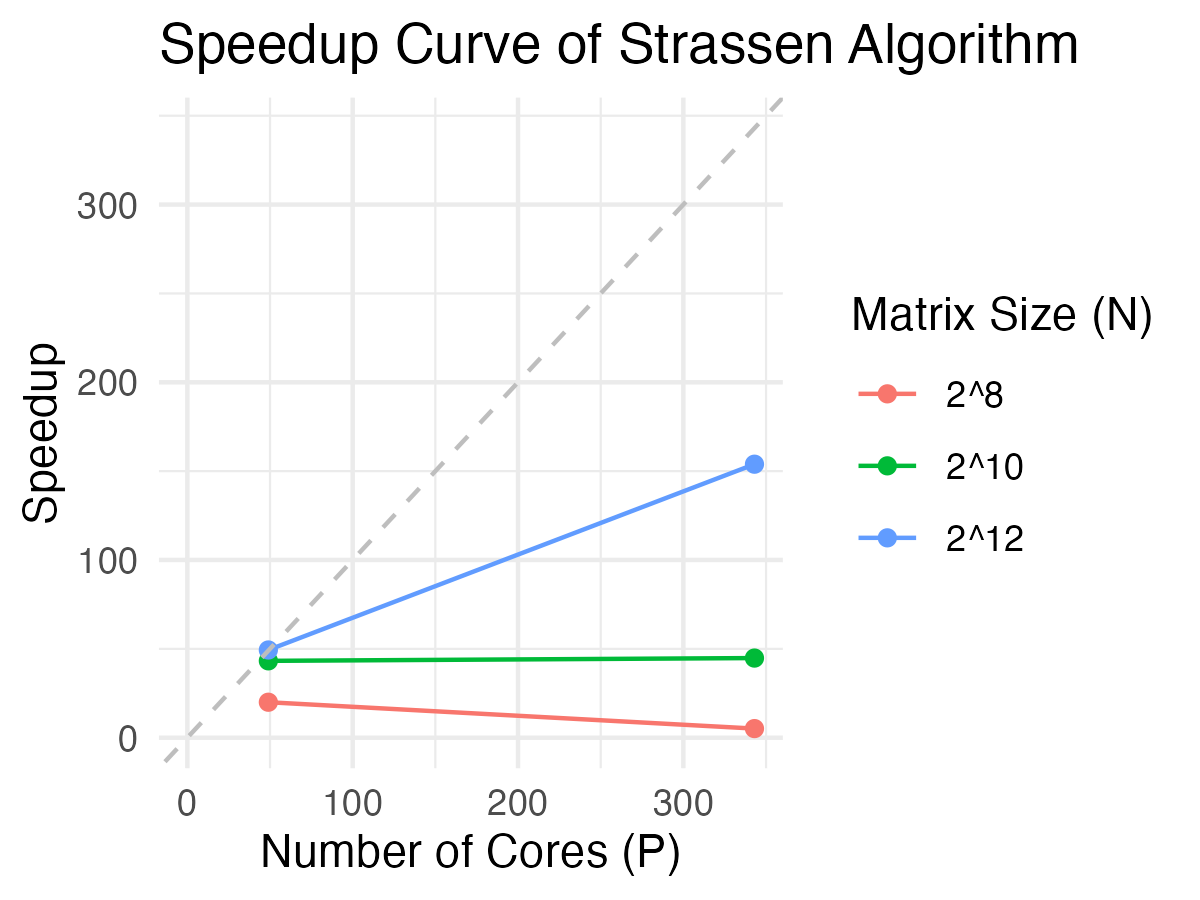
\includegraphics[width=0.5\textwidth]{speedup_curve.png}
    \caption{Speedup Curve for Matrix Sizes \( N \)}
    \label{fig:speedup_curve}
\end{figure}
    
For \( N = 2^8 \), the curve exhibits a normal speedup where \( S(P, N) < P \), 
 lying below the ideal diagonal. 
For \( N = 2^{10} \), the speedup closely follows the ideal diagonal, 
 indicating an almost perfect linear speedup. 
Interestingly, for \( N = 2^{12} \), the curve is above the diagonal, 
 suggesting a superlinear speedup, which is an rarel phenomenon.

\section{Analysis}

Overall, the parallel acceleration is remarkably significant. 
Interestingly, the speedup characteristics are not consistent across the 
 three matrix sizes \( N \). 
One intriguing observation is the superlinear speedup exhibited when 
 the matrix size is large (\( N = 2^{12} \)).
 
One hypothesis for this phenomenon is the cache effect. 
When \( N \) is relatively small, such as \( 2^8 \), 
 assuming each element of the matrices \( A \) and \( B \) occupies 4 bytes 
 as a floating-point number, 
 the combined space required for matrices would be 
 \( 2 \times 2^8 \times 2^8 \times 4 \) bytes, or 512 KB,
 which is not substantial. 
Such data could potentially be handled directly within the cache. 
As a result, the parallel computation exhibits a typical speedup, 
 with communication overheads significantly affecting performance.
 
However, for \( N = 2^{12} \), the combined space for matrices \( A \) and \( B \) becomes 
 \( 2 \times 2^{12} \times 2^{12} \times 4 \) bytes, or 128 MB.
This is a substantial amount of data, and excesses the cache size of most modern processors.
The total space rockets up, potentially preventing direct cache handling when computed with a single core. 
This would necessitate direct memory access, 
 significantly slowing down computation. 

Consequently, a nonlinear performance drop is observed 
 for single-core execution when transitioning from \( N = 2^{10} \) to \( N = 2^{12} \). 
In contrast, during parallel computation, each core only deals with a fraction of the matrix at a time. 
This fraction might still fit within the cache, 
 avoiding direct memory reads and substantially boosting speed. 
The drag due to communication overhead becomes relatively minimal in this scenario.

In conclusion, the observed performance benefits from the ring algorithm, especially in the $N=2^{12}$
case, highlight the potential impacts of faster memory hierarchies in parallel computing.

\appendix
\label{app:myappendix}
\section{Supplementary Tests}
To mitigate the influence of cache effects on the speedup results, 
 we redefined our baseline to \( P=4 \) and gathered results 
 using a different set of \( P \) values to plot the speedup curve.

\subsection{Performance}
\begin{table}[h]
    \centering
    \begin{tabular}{ccccccc}
        \toprule
        & \multicolumn{5}{c}{Ring Algorithm} & \multicolumn{1}{c}{} \\
        \cmidrule(lr){2-6}
        (in seconds) & \( P = 2^2 \) & \( P = 2^3 \) & \( P = 2^4 \) & \( P = 2^5 \) & \( P = 2^6 \) \\
        \midrule
        \( N = 2^8 \)  & 0.039433 & 0.020771 & 0.011038 & 0.009600 & 0.006572 \\
        \( N = 2^{10} \) & 2.123300 & 1.203297 & 0.635084 & 0.353849 & 0.175946 \\
        \( N = 2^{12} \) & 73.409207 & 37.168124 & 20.105683 & 10.941110 & 6.431338 \\
        \bottomrule
    \end{tabular}
    \caption{Updated performance of the Ring method.}
    \label{tab:updated_results}
\end{table}

Note that when we take \( P = 4 \) as the baseline, 
 the maxima data size for each processor shrink by a factor of 4, which is 32MB.
This is a more reasonable size for the cache, 
 and the performance is not expected to drop significantly as \( N \) increases.

\subsection{Updated Speedup}

With the updated performance data, we can compute the updated speedup values for each \( N \) 
based on the modified defination in Equation \ref{eqn:updated_speedup} with the performance results in Table \ref{tab:updated_results}.

\begin{equation}
    \label{eqn:updated_speedup}
    S(P, N) = 4 \times \frac{T(P,N)}{T(4, N)}
\end{equation}

The updated speedup values for each \( N \) are plotted in the following Figure \ref{fig:updated_speedup_curve}.

\begin{figure}[ht]
    \centering
    \includegraphics[width=0.5\textwidth]{speedup_curve_appendex.png}
    \caption{Updated Speedup Curve for Matrix Sizes \( N \)}
    \label{fig:updated_speedup_curve}
\end{figure}


\subsection{Analysis}
The updated speedup curve is much more consistent with regular speedup curves. 
All of the speedup values are below the ideal diagonal, with the speedup for \( N = 2^{12} \) and \( P = 2^{10} \)
 being above the speedup for \( N = 2^{8} \).

This suggests that when the matrix size is small, 
 the overhead of communication is significant, and the parallel computation becomes more effeicient 
 when the matrix size increases.

 In summary, while the updated speedup curve does exhibit benefits from parallel processing, 
  especially for larger matrices, 
  there remains a balance between computation and communication that 
  determines the overall performance gains.

\section*{File Notes}
The source code of the program is in the \texttt{project3} folder. 
For more details, please refer to the \texttt{README.md} file in the folder.

\end{document}


